\begin{tikzpicture}[]
  
  % Style for no padding
  \tikzset{no padding/.style={inner sep=0,outer sep=0}};
  
  \newlength{\plotheight}
  \setlength{\plotheight}{4cm}
  \newlength{\plotwidth}
  \setlength{\plotwidth}{7cm}
  \def \ymin {0.45}
  \def \ymax {1}
  \def \xmin {0}
  \def \xmax {\plotwidth}
  
  % Plot ytics defs
  \def \yticsfontsize {\scriptsize}
  \def \yticswidth {1mm}
  \tikzset{ytic/.style={anchor=east,inner xsep=0.75mm,xshift=-0mm}};
  \tikzset{y-help-line/.style={densely dotted,thin}};
  
  % Plot xtics defs
  \def \xticsfontsize {\scriptsize}
  \def \xticswidth {1mm}
  \tikzset{xtic/.style={anchor=base,inner ysep=0.75mm,yshift=-2mm}};
  
  % CStack width defs
  \newlength{\barwidth}
  \setlength{\barwidth}{0.041667\xmax}
  \newlength{\clusterwidth}
  \setlength{\clusterwidth}{6.000000\barwidth}
  \newlength{\padding}
  \setlength{\padding}{1.000000\barwidth}
  
  % Bar styles
  \tikzset{bone/.style={fill=black!10}};
  \tikzset{btwo/.style={fill=black!60}};
  \tikzset{bthree/.style={fill=white}};
  \tikzset{bfour/.style={fill=black}};
  
  % Legend defs
  \def \legendfontsize {\scriptsize}
  \tikzset{legend label/.style={anchor=base west,no padding}};
  \tikzset{legend node/.style={inner xsep=1mm,inner ysep=0.75mm,outer sep=0}};
  \def \legone {Baseline}
  \def \legtwo {Cool}
  \def \legthree {Very Cool}
  \def \legfour {Really Cool}
  
  % Outer box
  \draw [] (0, 0) rectangle (\plotwidth, \plotheight);
  
  % Plot area node
  \node (plotarea) at (0, 0)
    [anchor=south west,no padding] {
    \begin{tikzpicture}[xscale=1,yscale=7.2727272727272725]
      \draw [] (\xmin, \ymin) -- (\xmin, \ymin);
      \draw [] (\xmax, \ymax) -- (\xmax, \ymax);
      \draw [y-help-line] (\xmin, 0.5) -- (\xmax, 0.5);
      \draw [y-help-line] (\xmin, 0.55) -- (\xmax, 0.55);
      \draw [y-help-line] (\xmin, 0.6000000000000001) -- (\xmax, 0.6000000000000001);
      \draw [y-help-line] (\xmin, 0.65) -- (\xmax, 0.65);
      \draw [y-help-line] (\xmin, 0.7) -- (\xmax, 0.7);
      \draw [y-help-line] (\xmin, 0.75) -- (\xmax, 0.75);
      \draw [y-help-line] (\xmin, 0.8) -- (\xmax, 0.8);
      \draw [y-help-line] (\xmin, 0.8500000000000001) -- (\xmax, 0.8500000000000001);
      \draw [y-help-line] (\xmin, 0.9) -- (\xmax, 0.9);
      \draw [y-help-line] (\xmin, 0.95) -- (\xmax, 0.95);
      
      % Bars
      \def \base {\ymin}
      \draw [fill=white] (0\clusterwidth + \padding + 0\barwidth, \base) rectangle ++(\barwidth, 0.45 - \base);
      \draw [bone] (0\clusterwidth + \padding + 0\barwidth, \base) rectangle ++(\barwidth, 0.45 - \base);
      \draw [fill=white] (0\clusterwidth + \padding + 1\barwidth, \base) rectangle ++(\barwidth, 0.6 - \base);
      \draw [btwo] (0\clusterwidth + \padding + 1\barwidth, \base) rectangle ++(\barwidth, 0.6 - \base);
      \draw [fill=white] (0\clusterwidth + \padding + 2\barwidth, \base) rectangle ++(\barwidth, 0.65 - \base);
      \draw [bthree] (0\clusterwidth + \padding + 2\barwidth, \base) rectangle ++(\barwidth, 0.65 - \base);
      \draw [fill=white] (0\clusterwidth + \padding + 3\barwidth, \base) rectangle ++(\barwidth, 0.7 - \base);
      \draw [bfour] (0\clusterwidth + \padding + 3\barwidth, \base) rectangle ++(\barwidth, 0.7 - \base);
      \draw [fill=white] (1\clusterwidth + \padding + 0\barwidth, \base) rectangle ++(\barwidth, 0.7 - \base);
      \draw [bone] (1\clusterwidth + \padding + 0\barwidth, \base) rectangle ++(\barwidth, 0.7 - \base);
      \draw [fill=white] (1\clusterwidth + \padding + 1\barwidth, \base) rectangle ++(\barwidth, 0.87 - \base);
      \draw [btwo] (1\clusterwidth + \padding + 1\barwidth, \base) rectangle ++(\barwidth, 0.87 - \base);
      \draw [fill=white] (1\clusterwidth + \padding + 2\barwidth, \base) rectangle ++(\barwidth, 0.93 - \base);
      \draw [bthree] (1\clusterwidth + \padding + 2\barwidth, \base) rectangle ++(\barwidth, 0.93 - \base);
      \draw [fill=white] (1\clusterwidth + \padding + 3\barwidth, \base) rectangle ++(\barwidth, 0.97 - \base);
      \draw [bfour] (1\clusterwidth + \padding + 3\barwidth, \base) rectangle ++(\barwidth, 0.97 - \base);
      \draw [fill=white] (2\clusterwidth + \padding + 0\barwidth, \base) rectangle ++(\barwidth, 0.8 - \base);
      \draw [bone] (2\clusterwidth + \padding + 0\barwidth, \base) rectangle ++(\barwidth, 0.8 - \base);
      \draw [fill=white] (2\clusterwidth + \padding + 1\barwidth, \base) rectangle ++(\barwidth, 0.9 - \base);
      \draw [btwo] (2\clusterwidth + \padding + 1\barwidth, \base) rectangle ++(\barwidth, 0.9 - \base);
      \draw [fill=white] (2\clusterwidth + \padding + 2\barwidth, \base) rectangle ++(\barwidth, 0.94 - \base);
      \draw [bthree] (2\clusterwidth + \padding + 2\barwidth, \base) rectangle ++(\barwidth, 0.94 - \base);
      \draw [fill=white] (2\clusterwidth + \padding + 3\barwidth, \base) rectangle ++(\barwidth, 0.99 - \base);
      \draw [bfour] (2\clusterwidth + \padding + 3\barwidth, \base) rectangle ++(\barwidth, 0.99 - \base);
      \draw [fill=white] (3\clusterwidth + \padding + 0\barwidth, \base) rectangle ++(\barwidth, 0.91 - \base);
      \draw [bone] (3\clusterwidth + \padding + 0\barwidth, \base) rectangle ++(\barwidth, 0.91 - \base);
      \draw [fill=white] (3\clusterwidth + \padding + 1\barwidth, \base) rectangle ++(\barwidth, 0.95 - \base);
      \draw [btwo] (3\clusterwidth + \padding + 1\barwidth, \base) rectangle ++(\barwidth, 0.95 - \base);
      \draw [fill=white] (3\clusterwidth + \padding + 2\barwidth, \base) rectangle ++(\barwidth, 0.96 - \base);
      \draw [bthree] (3\clusterwidth + \padding + 2\barwidth, \base) rectangle ++(\barwidth, 0.96 - \base);
      \draw [fill=white] (3\clusterwidth + \padding + 3\barwidth, \base) rectangle ++(\barwidth, 1.0 - \base);
      \draw [bfour] (3\clusterwidth + \padding + 3\barwidth, \base) rectangle ++(\barwidth, 1.0 - \base);
    \end{tikzpicture}
  };
  \node (legend) at (plotarea.north west)
    [anchor=north west,draw,fill=white,inner xsep=1mm,inner ysep=0.75mm,outer sep=0,xshift=1mm,yshift=-1mm] {
    \begin{tikzpicture}[]
      \node (legone-node) at (0,0)
        [anchor=west,legend node] {
        \begin{tikzpicture}[]
          \node at (0,0) [legend label] {\legendfontsize{\legone\vphantom{yg}}};
          \draw [bone] (-1mm, 0mm) rectangle ++(-2mm, 2mm);
        \end{tikzpicture}
      };
      \node (legtwo-node) at (legone-node.east)
        [anchor=west,legend node] {
        
\begin{tikzpicture}[]
          \node at (0,0) [legend label] {\legendfontsize{\legtwo\vphantom{yg}}};
          \draw [btwo] (-1mm, 0mm) rectangle ++(-2mm, 2mm);
        \end{tikzpicture}
      };
      \node (legthree-node) at (legtwo-node.east)
        [anchor=west,legend node] {
        
\begin{tikzpicture}[]
          \node at (0,0) [legend label] {\legendfontsize{\legthree\vphantom{yg}}};
          \draw [bthree] (-1mm, 0mm) rectangle ++(-2mm, 2mm);
        \end{tikzpicture}
      };
      \node (legfour-node) at (legthree-node.east)
        [anchor=west,legend node] {
        
\begin{tikzpicture}[]
          \node at (0,0) [legend label] {\legendfontsize{\legfour\vphantom{yg}}};
          \draw [bfour] (-1mm, 0mm) rectangle ++(-2mm, 2mm);
        \end{tikzpicture}
      };
    \end{tikzpicture}
  };
  \node (ytics) at (0, 0)
    [anchor=south east,no padding] {
    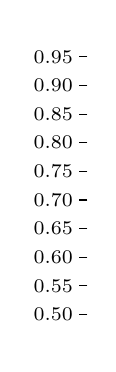
\begin{tikzpicture}[yscale=7.2727272727272725]
      \draw [] (0, \ymin) -- (0, \ymin);
      \draw [] (0, \ymax) -- (0, \ymax);
      \draw [] (0, 0.5) -- ++(-\yticswidth,0);
      \node at (-\yticswidth, 0.5) [ytic] {\yticsfontsize{0.50}};
      \draw [] (0, 0.55) -- ++(-\yticswidth,0);
      \node at (-\yticswidth, 0.55) [ytic] {\yticsfontsize{0.55}};
      \draw [] (0, 0.6000000000000001) -- ++(-\yticswidth,0);
      \node at (-\yticswidth, 0.6000000000000001) [ytic] {\yticsfontsize{0.60}};
      \draw [] (0, 0.65) -- ++(-\yticswidth,0);
      \node at (-\yticswidth, 0.65) [ytic] {\yticsfontsize{0.65}};
      \draw [] (0, 0.7) -- ++(-\yticswidth,0);
      \node at (-\yticswidth, 0.7) [ytic] {\yticsfontsize{0.70}};
      \draw [] (0, 0.75) -- ++(-\yticswidth,0);
      \node at (-\yticswidth, 0.75) [ytic] {\yticsfontsize{0.75}};
      \draw [] (0, 0.8) -- ++(-\yticswidth,0);
      \node at (-\yticswidth, 0.8) [ytic] {\yticsfontsize{0.80}};
      \draw [] (0, 0.8500000000000001) -- ++(-\yticswidth,0);
      \node at (-\yticswidth, 0.8500000000000001) [ytic] {\yticsfontsize{0.85}};
      \draw [] (0, 0.9) -- ++(-\yticswidth,0);
      \node at (-\yticswidth, 0.9) [ytic] {\yticsfontsize{0.90}};
      \draw [] (0, 0.95) -- ++(-\yticswidth,0);
      \node at (-\yticswidth, 0.95) [ytic] {\yticsfontsize{0.95}};
    \end{tikzpicture}
  };
  \node (xtics) at (0, 0)
    [anchor=north west,no padding] {
    
\begin{tikzpicture}[xscale=1]
      \draw [] (\xmin, 0) -- (\xmin, 0);
      \draw [] (\xmax, 0) -- (\xmax, 0);
      \draw [] (0.500000\clusterwidth, 0) -- ++(0,-\xticswidth);
      \node at (0.500000\clusterwidth, -\xticswidth) [xtic] {\xticsfontsize{bench1}};
      \draw [] (1.500000\clusterwidth, 0) -- ++(0,-\xticswidth);
      \node at (1.500000\clusterwidth, -\xticswidth) [xtic] {\xticsfontsize{bench2}};
      \draw [] (2.500000\clusterwidth, 0) -- ++(0,-\xticswidth);
      \node at (2.500000\clusterwidth, -\xticswidth) [xtic] {\xticsfontsize{bench3}};
      \draw [] (3.500000\clusterwidth, 0) -- ++(0,-\xticswidth);
      \node at (3.500000\clusterwidth, -\xticswidth) [xtic] {\xticsfontsize{bench4}};
    \end{tikzpicture}
  };
\end{tikzpicture}